\subsection{Process change exploration}\label{sec:3c:pce}


% as has been shown the prediction is nice but it is difficult to derive the insignts 
% definition of the visualization
% humans cannot comprehend the results and we need visualzation 
% (new functions on vis that ar enot mentioned before should be mentioned?)

%%%
% outline:
% 0. short intro
% 1. user tasks
% 2. design (and what supports design)
% 3. implementation and the resources.
%%%

In~\Cref{sec:3a:preliminaries} and \Cref{sec:3b:df} we described the approach for forecasting process models. To that end, gaining actual insights from such predicted values remains a difficult task for the analyst. This section sets off to present the design of a novel visualisation system to aid analysts in the exploration of the event logs and their corresponding (forecasted) discovered process models.

Following the user tasks~\ref{req:adaptation} and~\ref{req:interactive} from~\Cref{sec:2:motivation}, we designed a Process Change Exploration (PCE) system to support the interpretation of the process model forecasts. PCE is an interactive visualisation system that consists of three connected views.


%In order to design the system we first established user tasks as a basis for the system design decisions. 


%To derive the user tasks we focus on the requirements of process mining analysis with respect to process forecasting and visualization principles. The authors of~\cite{DBLP:conf/bpm/PollPRRR18} discuss the opportunities for process forecasting. They describe that the utility of process forecasting is an understanding of the incremental changes or adaptations that happen to the process model into the future. In designing an explorative visualization system, we also followed the "Visual Information-Seeking Mantra:"~\emph{overview first, zoom and filter, then details-on-demand}~\cite{DBLP:conf/vl/Shneiderman96}. 
%%(maybe talk about tasks? not requirements)
%Thus, we expect the design of our system to assist in the following tasks:
%
%%requirements for the visualization based on the related literature and experience working with event sequence data. 
%
%\begin{requidescr}
%	\item[Identify process adaptations:\namedlabel{req:adaptation}] The visualization system should assist the user in identifying the changes that happen in the process model of the future in respect to the past;
%	\item[Allow for interactive exploration:\namedlabel{req:interactive}] The user should be able to follow the visual information-seeking principles, including overview first, filtering, zooming, details-on-demand principles.;
%\end{requidescr} % CUSTOM from CDC, with love :)




\textbf{Adaptation Directly-Follows Graph (aDFG) view.} This is the main view of the visualisation that will show the model of the process. In order to accomplish task~\ref{req:adaptation}, we modify the DFG syntax. In order to display the process model adaptation from time range $T_{i_0}-T_{j_0}, i_0<j_0$ to $T_{i_1}-T_{j_1}, i_1<j_1$ we display the union of the process models of these regions, annotating the nodes and edges with the numbers of both ranges. We colour the aDFG as follows: we use colour saturation to show the nodes with higher values. We colour edges with a diverging saturation (red-black-green) schema. This colouring applies red colour to edges that are dominant in the $T_{i_0}-T_{j_0}$ range, and green if edges are dominant in the $T_{i_1}-T_{j_1}$ range, otherwise the edge is close to black. For coloring edges, we used idea of the three colour schema from~\cite{DBLP:conf/grapp/KriglsteinR12}.

\textbf{Timeline view with brushed regions.} This view represents the area chart graph that shows how the number of activity executions change with time. The area chart colour is split in two parts, one for the actual data, and the other one to show the time range where values are predicted. Analysts can brush one region in order to zoom in, creating one region of interest $T_{i_0,}-T_{j_0}, i_0<j_0$ that is displayed on the DFG. Analyst can also brush two regions of the area chart to select two time ranges, updating the DFG to aDFG representation. The brushed regions are coloured accordingly to the schema for colouring aDFG transitions. The earlier brushed region is coloured in red, while the second one is coloured green. 

\textbf{Activity and path sliders.} We adopt two sliders that are used to simplify the DFG~\cite{leemans2019directly} and the aDFG for detailed exploration of the models.

Based on the described views, we conjecture that the analyst is able to accomplish the tasks~\ref{req:adaptation}, and~\ref{req:interactive} with ease.



%The interactive system consists of three parts. Part b shows the timeline of the data (green region), and forecasted values (grey region). The user can brush one or two regions (in this b.1 and b.2) on this graph to see the filtered for that time range process model or a difference between two process models. The main view (a) represents the directly follows change graph that shows the difference between two brushed regions. The c.1 and c.2 are the usual filters on the number of paths and activities to aid simplification the visual representation




%\begin{figure}
%	\centering
%	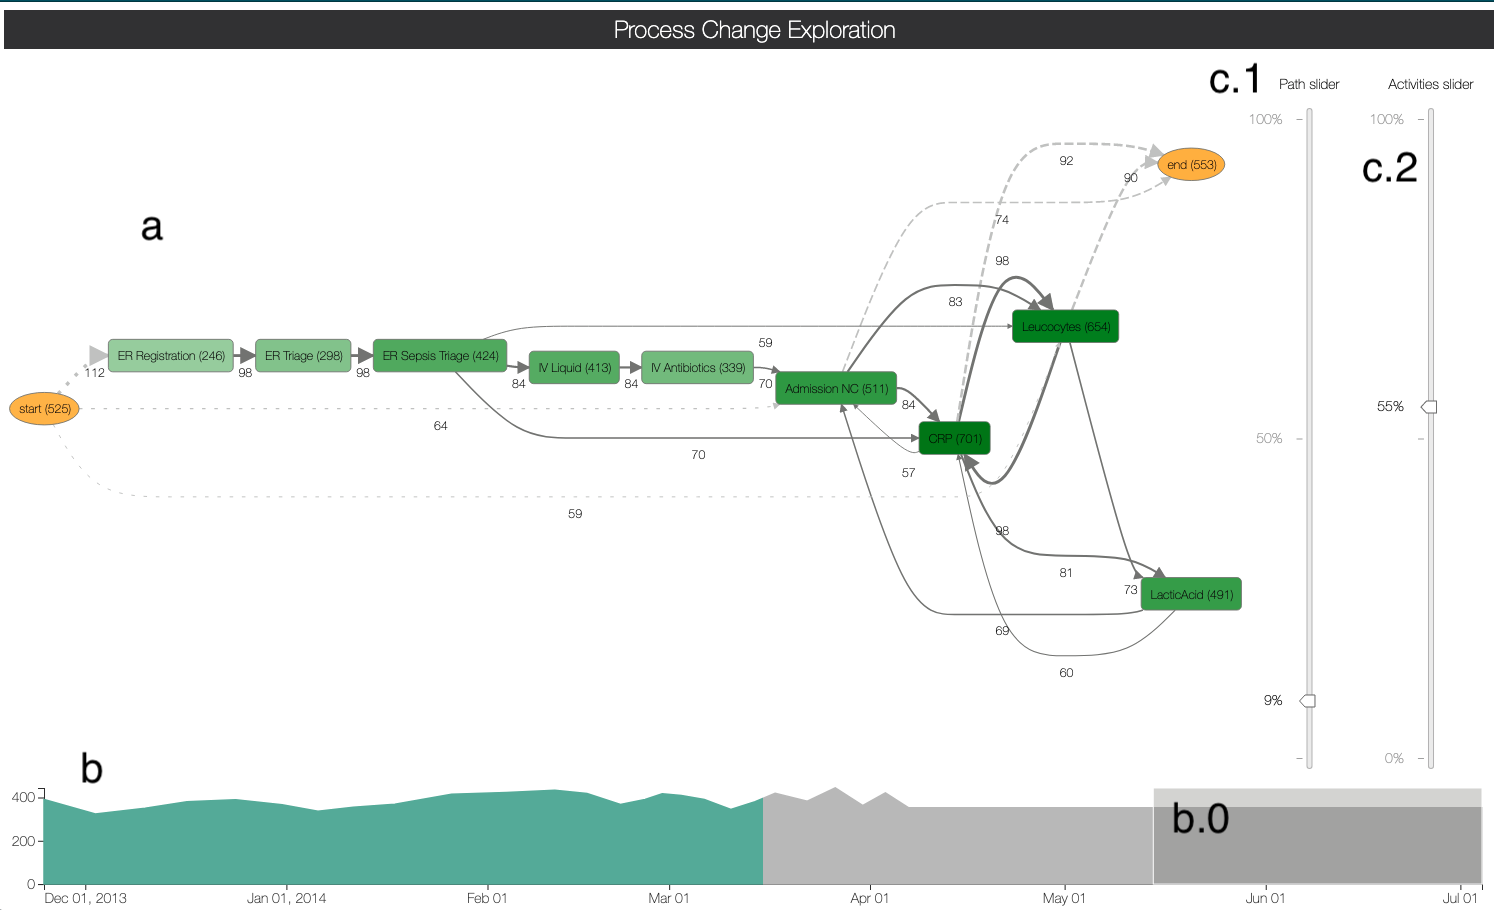
\includegraphics[width=\textwidth]{img/vis/vis-system-one-brush.png}
%	\caption{Process Change Exploration (PCE) system.} 
%	\label{fig:vis-one-brushes}
%\end{figure}

%Process Change Exploration (PCE) system. The interactive system consists of three parts. Part b shows the timeline of the data (green region), and forecasted values (grey region). The user can brush one time range (in this b.0) on this graph to see the filtered for that time range process model. The main view (a) represents the directly follows graph of that region. The c.1 and c.2 are the usual filters on the number of paths and activities to aid simplification the visual representation}

%
%\noindent\textbf{%
%Implementation. 
%} 


%\noindent\textbf{%
%	User interface
%} The Figure~\ref{fig:vis-two-brushes} displays the screenshot of the PCE visualization system. 
%We improve upon the notion of Directly-Follows graph~\cite{leemans2019directly} that is widely used in process mining research and practice. We use the ideas from the version graph~\cite{DBLP:conf/grapp/KriglsteinR12} on how to represent the change between versions of the graph with coloring of the transitions. 



% as has been shown the prediction is nice but it is difficult to derive the insignts 
% definition of the visualization
% humans cannot comprehend the results and we need visualzation 
% (new functions on vis that ar enot mentioned before should be mentioned?)

%%%
% outline:
% 0. short intro
% 1. user tasks
% 2. design (and what supports design)
% 3. implementation and the resources.
%%%